\subsection{Energy Bandy in Solids} \label{chap2}

\subsubsection*{Electron of Bloch}
Independent electrons which obey the one electron Schrödinger equation for a periodic potential are called Bloch
electrons and obey Bloch’s theorem. Own functions of $\Psi_k(r)$ of the Hamiltonian in the field perfectly ideally periodic crystal lattice can be presented in the form of:
\begin{equation}
\Psi_k(r) = u_k(r)exp(ik \cdot r)
\end{equation}
, where $u_k(r)$ is a function with periodicity of the network, i.e.
\begin{equation}
u_k(r) = u_k(r + R_n)
\end{equation}
for all Bravais $R_n$ vectors. Note that from the above formulas it follows that
$$
\Psi_k(r+R_n) =  u_k(r)exp[ik\cdot(r+Rn)]= \Psi_k(r)expik\cdot R_n)
$$
This relationship allows an alternative formulation of Bloch's theorem: own functions
Hamiltonian, a perfectly periodic crystal lattice can be represented in such a way that each
of them corresponded to a certain wave vector k, with
$$
\Psi_k(r+R_n) = \Psi_k(r)exp(ik \cdot R_n)
$$
Bloch's theorem makes it easier to determine the electron's wave functions in a crystal, because that's enough
be limited to one unit cell, while the original wave function in the equation
Schrödinger applies to the whole crystal.

\subsubsection*{Band Dispersion compared to Free Electro Model}

The free electron model allows to describe, for example,
specific heat, thermal conductivity and thermal expansion. This model, however, does not include where observed differences come from between metals, semiconductors and insulators. To this end, necessary
is to take into account the periodic structure of the crystal, which leads to periodically changing
potential in which the electrons move in the crystal. The most important feature of the extended
the model is the prediction of electron energy bands,
separated by gaps . The crystal is an insulator when the allowed energy bands are completely empty
or completely planted. If one of the permitted bands is partially filled, then
the crystal behaves like a metal. Where one or two bands are planted only in
slightly or very little crystal is a semiconductor

\begin{figure}[H]
  \centering
  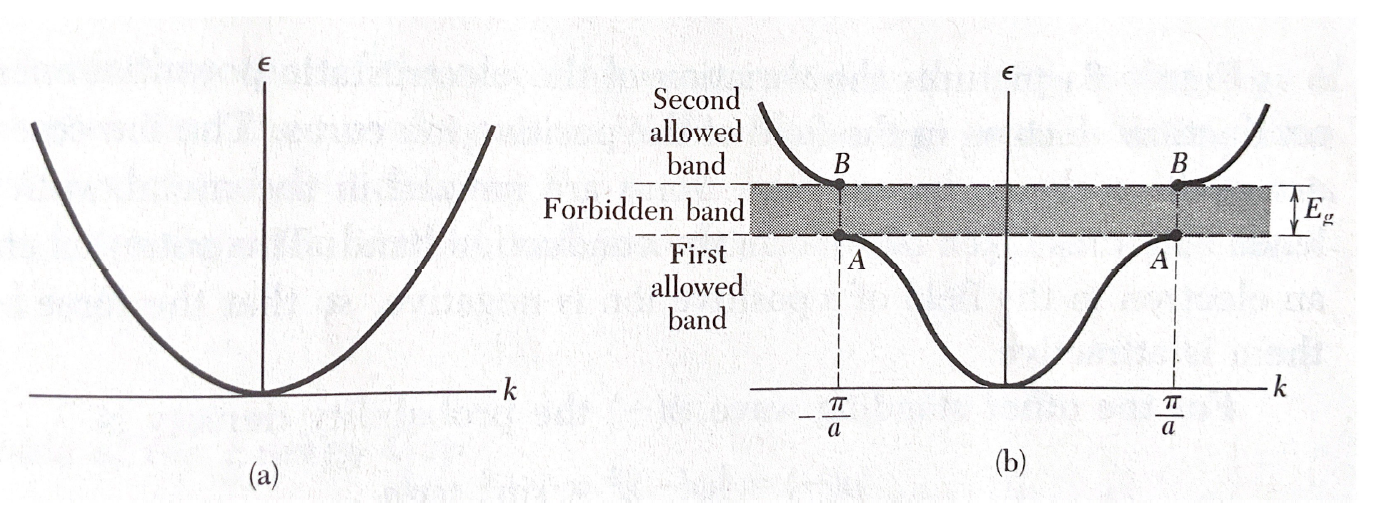
\includegraphics[width=0.6\linewidth]{Graphics/Chapter2/ek_allowed.png}
  \caption{(a) Plot of energy $\varepsilon$ versus wavevector $k$ for a free electron. (b) Plot of energy versus wavevector for an electron in a monoatomic
  linear lattice of lattice constant $a$. The energy gap $E_g$ shown is associated with the first Bragg reflection as $k=\pm \pi/a$; other gaps 
  are found at $k=\pm n\pi/a$, for integral values of $n$.
  \cite[Introduction to  Solid State Physics p. 177]{kittel} }
  \label{fig:ek_allowed}
\end{figure}

\autoref{fig:ek_allowed} these gaps are shwon, as it are energy level
which are not allowed for the electrons.

\subsubsection*{Velocity of Bloch Electron}

The the given energy of an electron of Bloch 

$$E(k) =  -E_0\left[\cos(k_xa)+1\right]$$ 
 
the velocity can be calculated by the following equation.

$$\vec{v} = \frac{1}{\hbar} \nabla_k E(\vec{k})$$

Which leads to the following eqation for the velocity

$$v_x = \frac{1}{h\hbar} \frac{d}{dk_x} -E_0\left[\cos(k_xa)+1\right] = \frac{E_0a}{h} \sin(k_xa)$$

As for the mass follows from:

$$E = \frac{\hbar^2k^2}{2m^*} \quad \rightarrow \qquad m^* = \frac{\hbar k_x}{v_x}  = \frac{k_x}{\sin(k_xa)} \cdot \frac{h}{E_0a}$$

For $E_0 = 1$ and $a=1$ the graphs are shown in the following.

\begin{figure}[H]
    \centering
    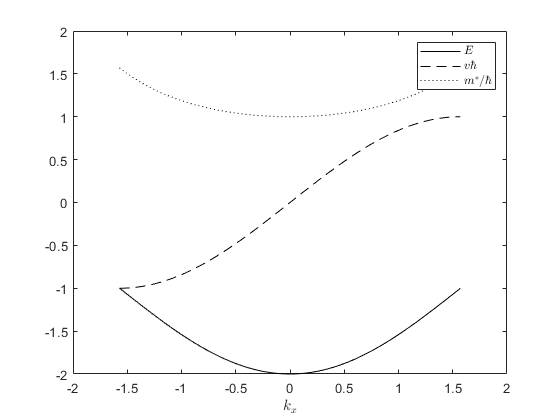
\includegraphics[width=0.5\linewidth]{Graphics/Chapter2/E_of_K.png}
    \caption{Energy, Velocity in x direction and reduced mass as a funktion of k}
    \label{fig:PNjunction}
  \end{figure}
